\documentclass{article}
\usepackage{graphicx}
\usepackage{amsmath}
\usepackage{caption}
\usepackage[utf8]{inputenc}

\title{Analisi dell'impatto di "bias" e topologia sui tempi di assorbimento per Dinamiche di Opinioni}
\author{Biancone Saverio}
\date{Ottobre 2020}

\begin{document}

\maketitle

\section{Introduzione}
[ALLA FINE]
\section{La dinamica delle opinioni}
La dinamica delle opinioni ha come obiettivo quello di sviluppare dei modelli matematici volti a descrivere l'evoluzione delle opinioni all'interno di una rete sociale formata da individui interagenti.\\*
Tali studi hanno portato allo sviluppo di numerosi modelli, adottando caratteristiche diversificate per quanto riguarda le dinamiche di interazione e il numero delle opinioni prese in esame, che hanno trovato come campo di applicazione discipline che vanno dalle Scienze Sociali alla Fisica e alla Biologia.
\subsection{Lo studio}
Il modello preso in esame descrive un sistema binario che prevede l'esistenza di due opinioni adottabili, indicate d'ora in poi con opinione 0 e opinione 1. Gli individui del sistema esprimeranno una preferenza verso una delle due opinioni, che definiremo  dominante\footnote{la definizione di opinione dominante dipende dal contesto ed esula dagli obiettivi di questo scritto}.\\*
Senza perdita di generalità assumeremo 1 come tale.\\*
Il sistema evolve in passi. Inizialmente ogni individuo condivide l'opinione 0.\\*
Ad ogni passo, un individuo scelto casualmente adotta l'opinione 1 (dominante) con probabilità $\alpha$, mentre con probabilità 1-$\alpha$ adotta una delle due opinioni possibili attraverso una delle dinamiche prestabilite.\\*
Le dinamiche di aggiornamento dell'opinione prese in considerazione sono:
\begin{itemize}
\item $Voter$ $Model$, nel quale l'individuo adotterà l'opinione di uno dei suoi vicini scelto casualmente
\item $Majority$ $Dynamic$, nel quale l'individuo adotterà l'opinione più diffusa tra i suoi vicini. In caso di parità verrà scelta una delle due opinioni con probabilità uniforme.
\end{itemize}
L'obiettivo è quello di analizzare il numero di passi, in valore atteso, necessari affinchè si raggiunga il consenso verso l'opinione dominante. È facile notare come, raggiunto questo stato, il sistema non possa evolvere più. Definiremo perciò tale stato "Stato di Assorbimento".\\*
Tale analisi è volta a rivelare, qualora esistesse, il legame che intercorre tra la topologia della rete e il numero di passi necessari a raggiungere lo stato di assorbimento, sotto una specifica dinamica.
La dinamica di aggiornamento dell'opinione principalmente trattata in questo lavoro è Majority-Dynamic.

\subsection{Lo stato dell'arte}
Nel corso degli anni sono stati molteplici gli studi riguardanti la Dinamica delle Opinioni, in particolare per quanto concerne l'impatto che differenti modelli e topologie hanno sul raggiungimento del consenso.\\*
Il mio lavoro si pone come integrazione del paper "Biased Opinion Dynamics: When the Devil is in the Details" [1], con cui condivide il modello, ed ha come fine ultimo quello di rispondere ad alcuni quesiti lasciati insoluti, attraverso un'analisi dei dati ottenuti simulando il processo descritto nel paragrafo precedente.
Il Voter-Moder ricopre un ruolo secondario nel mio lavoro, in quanto già dimostrato nel paper [1] che il tempo di assorbimento nel modello preso in esame è di $O(\frac{1}{\alpha}n\log{}n)$ passi con altà probabilità, indipendentemente dalla topologia della rete.\\*
Differenti invece sono i legami, come dimostrato, che intercorrono tra il "bias", la topologia e il tempo di assorbimento quando la dinamica di aggiornamento è Majority-Dynamic.\\*
In un Ciclo di $n$ nodi il consenso viene raggiunto in $O(\frac{1}{\alpha}n\log{}n)$ passi in valore atteso, mentre su topologie più dense con grado minimo $\Omega(\log{}n)$, il tempo di assorbimento è $O(n\log{}n)$ fino a chè il bias è $\geq$ $\frac{1}{2}$.


\section{Studi svolti e Analisi dei risultati}
Basandomi sui risultati descritti dal paper [1] e riportati nel precedente capitolo, ho tentato di rispondere ad alcune delle domande rimaste insolute.\\*
La mia attenzione è stata rivolta in particolare al tempo di assorbimento che si ottiene adottando Majority-Dynamic su alcune topologie quando il bias è inferiore a $\frac{1}{2}$.\\*
Per poter comparare ed analizzare statisticamente i tempi di assorbimento, ho sviluppato un software in grado di simulare il modello preso in esame sulle seguenti topologie:
 \begin{itemize}
\item Ipercubo
\item Clique
\item Ciclo
\item Modello di Erdős–Rényi G($n$,$p$)
\end{itemize}
\subsection{Analisi di Clique, Ipercubo e Ciclo}
I primi test eseguiti sono serviti a verificare l'accuratezza del software e correggerne eventuali errori. Ogni test è composto da 100 simulazioni, configurate con Majority-Dynamic e bias pari a $\frac{1}{2}$.\\*
I test sono stati eseguiti su Ipercubi, Cliques e Cicli, in dimensioni che vanno da $2^{5^{\mathrm{}}}$ fino a $2^{12^{\mathrm{}}}$ vertici.\\*
\begin{center}
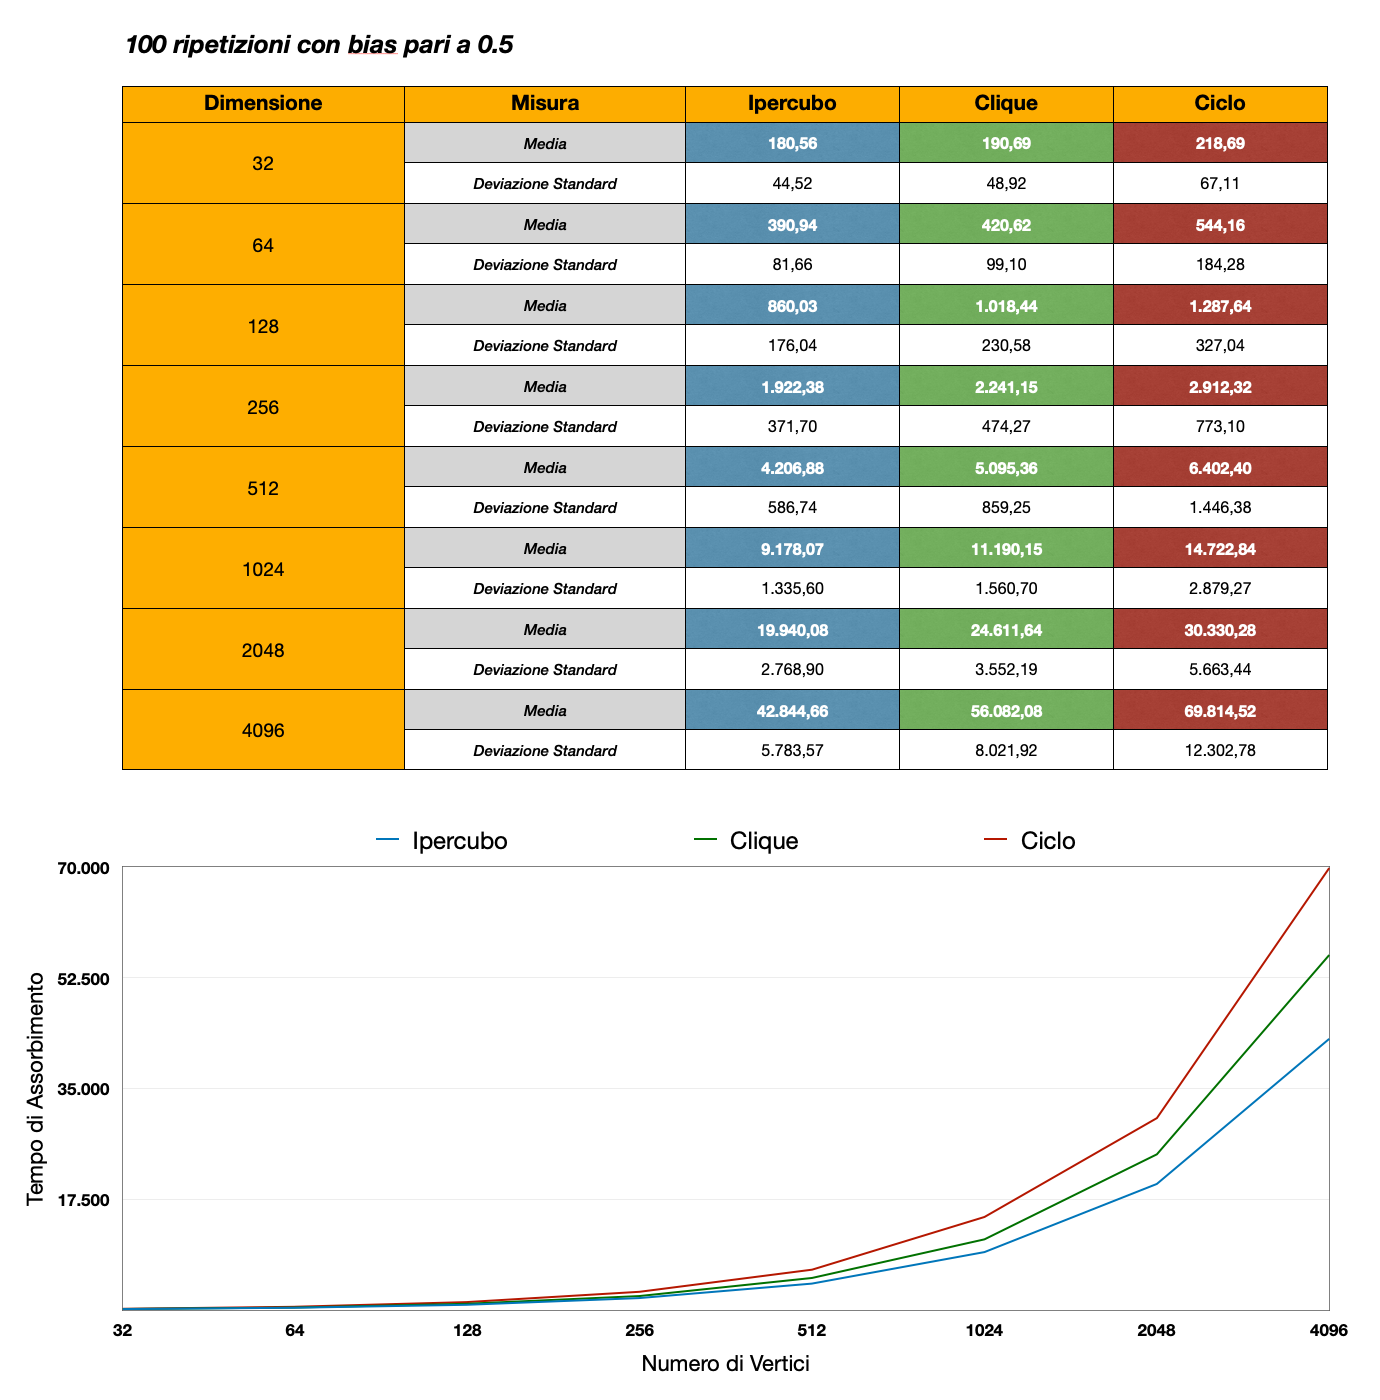
\includegraphics[width=1\textwidth]{Test/test_bias05.png}
\end{center}
I risultati ottenuti sono perfettamente in linea con quanto dimostrato teoricamente in  "Biased Opinion Dynamics" [1]. Per quanto riguarda il Ciclo, il tempo di assorbimento è stato pari a $O(\frac{1}{\alpha}n\log{}n)$. \\*
Riguardo Clique e Ipercubo, per i quali il grado minimo è pari a $\Omega(\log{}n)$, il tempo di assorbimento con bias pari a $\frac{1}{2}$ si è rivelato essere $O(n\log{}n)$, anche questa volta confermando quanto evidenziato dal paper [1].\\*
Una volta appurato perciò che il software simulasse correttamente i processi descritti, ottenendo risultati conformi a quanto atteso, sono stati eseguiti test metodologicamente analoghi ai precedenti, adottando però un bias verso l'opinione dominante pari a $\frac{1}{4}$, di fatto dimezzandolo.\\*
\begin{center}
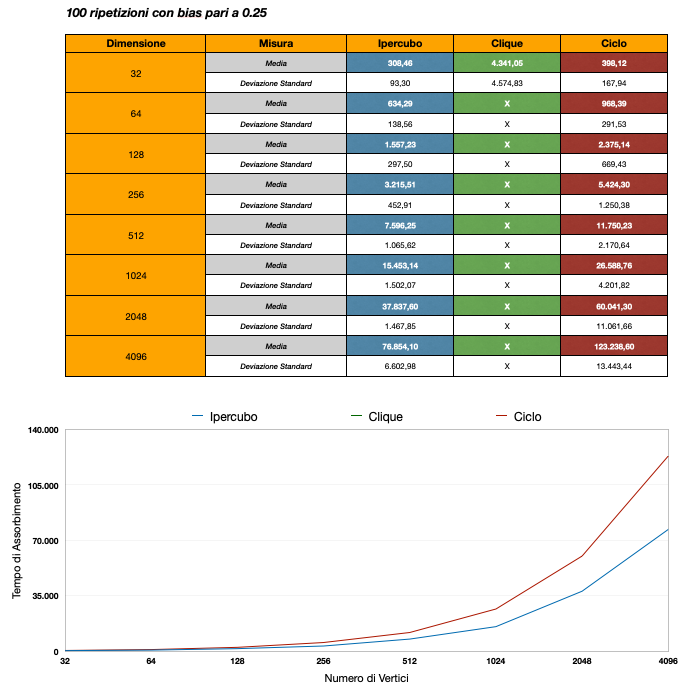
\includegraphics[width=1\textwidth]{Test/test_bias025.png}
\end{center}
Per quanto riguarda il Ciclo e la Clique, sono stati ancora una volta confermati i risultati attesi.
Lo stato di assorbimento per il Ciclo è stato nuovamente raggiunto in $O(\frac{1}{\alpha}n\log{}n)$ passi in valore atteso. Nello specifico, dimezzando il valore del bias, i tempi di assorbimento per tale topologia sono raddoppiati, suggerendo una proporzionalità inversa tra il tempo di assorbimento e il valore del bias.\\*
D'altra parte, come previsto, è stato impossibile ultimare i test per la Clique, in quanto, con un bias inferiore a $\frac{1}{2}$, il numero di passi necessari a raggiungere lo stato di assorbimento è diventato esponenziale nel grado minimo ($n-1$ per le Clique), di fatto rendendo impossibile lo svolgimento dei test già dalla dimensione di $2^{6^{\mathrm{}}}$.\\*
Il paper in esame [1], d'altronde, lascia aperta la domanda inerente al comportamento dell'Ipercubo con un bias così basso. Dal risultato dei test si evince come l'Ipercubo abbia un comportamento assimilabile a quello del Ciclo, raggiungendo perciò lo stato di assorbimento in $O(n\log{}n)$ passi.
\subsection{Analisi del Modello di Erdős–Rényi}
Questa sezione è dedicata all'analisi dei tempi di assorbimento per topologie non regolari, cioè grafi per i quali i vertici non condividono lo stesso grado.\\
Tali topologie sono state generate scrivendo un algoritmo aleatorio basato sul Modello di Erdős–Rényi G($n$,$p$).\\*
In tale modello, dato un grafo G($V$,$E$) con $|V|$ = $n$,
\begin{equation}
    \forall \: u,v \in V,\; (u,v) \in E  \text{ con probabilità } p.
\end{equation}
I test eseguiti sono composti da 100 simulazioni, configurate con Majority-Dynamic e bias pari a $\frac{1}{4}$.\\*
Le topologie prese in considerazione hanno dimensioni che vanno da $2^{5^{\mathrm{}}}$ fino a $2^{12^{\mathrm{}}}$ vertici e sono state generate con il modello G($n$,$p$) descritto precedentemente, utilizzando i seguenti valori di $p$:
\begin{itemize}
\item $p$ $\leq$ $\frac{1-\epsilon}{n}$, per il quale il grafo risulta principalmente sparso, con alta probabilità
\item $p$ $\geq$ $\frac{1+\epsilon}{n}$, per il quale il grafo presenta una $giant$ $component$ circondata da componenti più piccole di dimensione $O(\log{}n)$, con alta probabilità
\item $p$ = $\frac{\log{}n}{n}$, per il quale il grafo risulta connesso e discretamente denso, con alta probabilità
\end{itemize}
Esempi: $n$ = 256, $\epsilon$ = $\frac{1}{2}$
\begin{figure}[!htb]
\minipage{0.31\textwidth}
  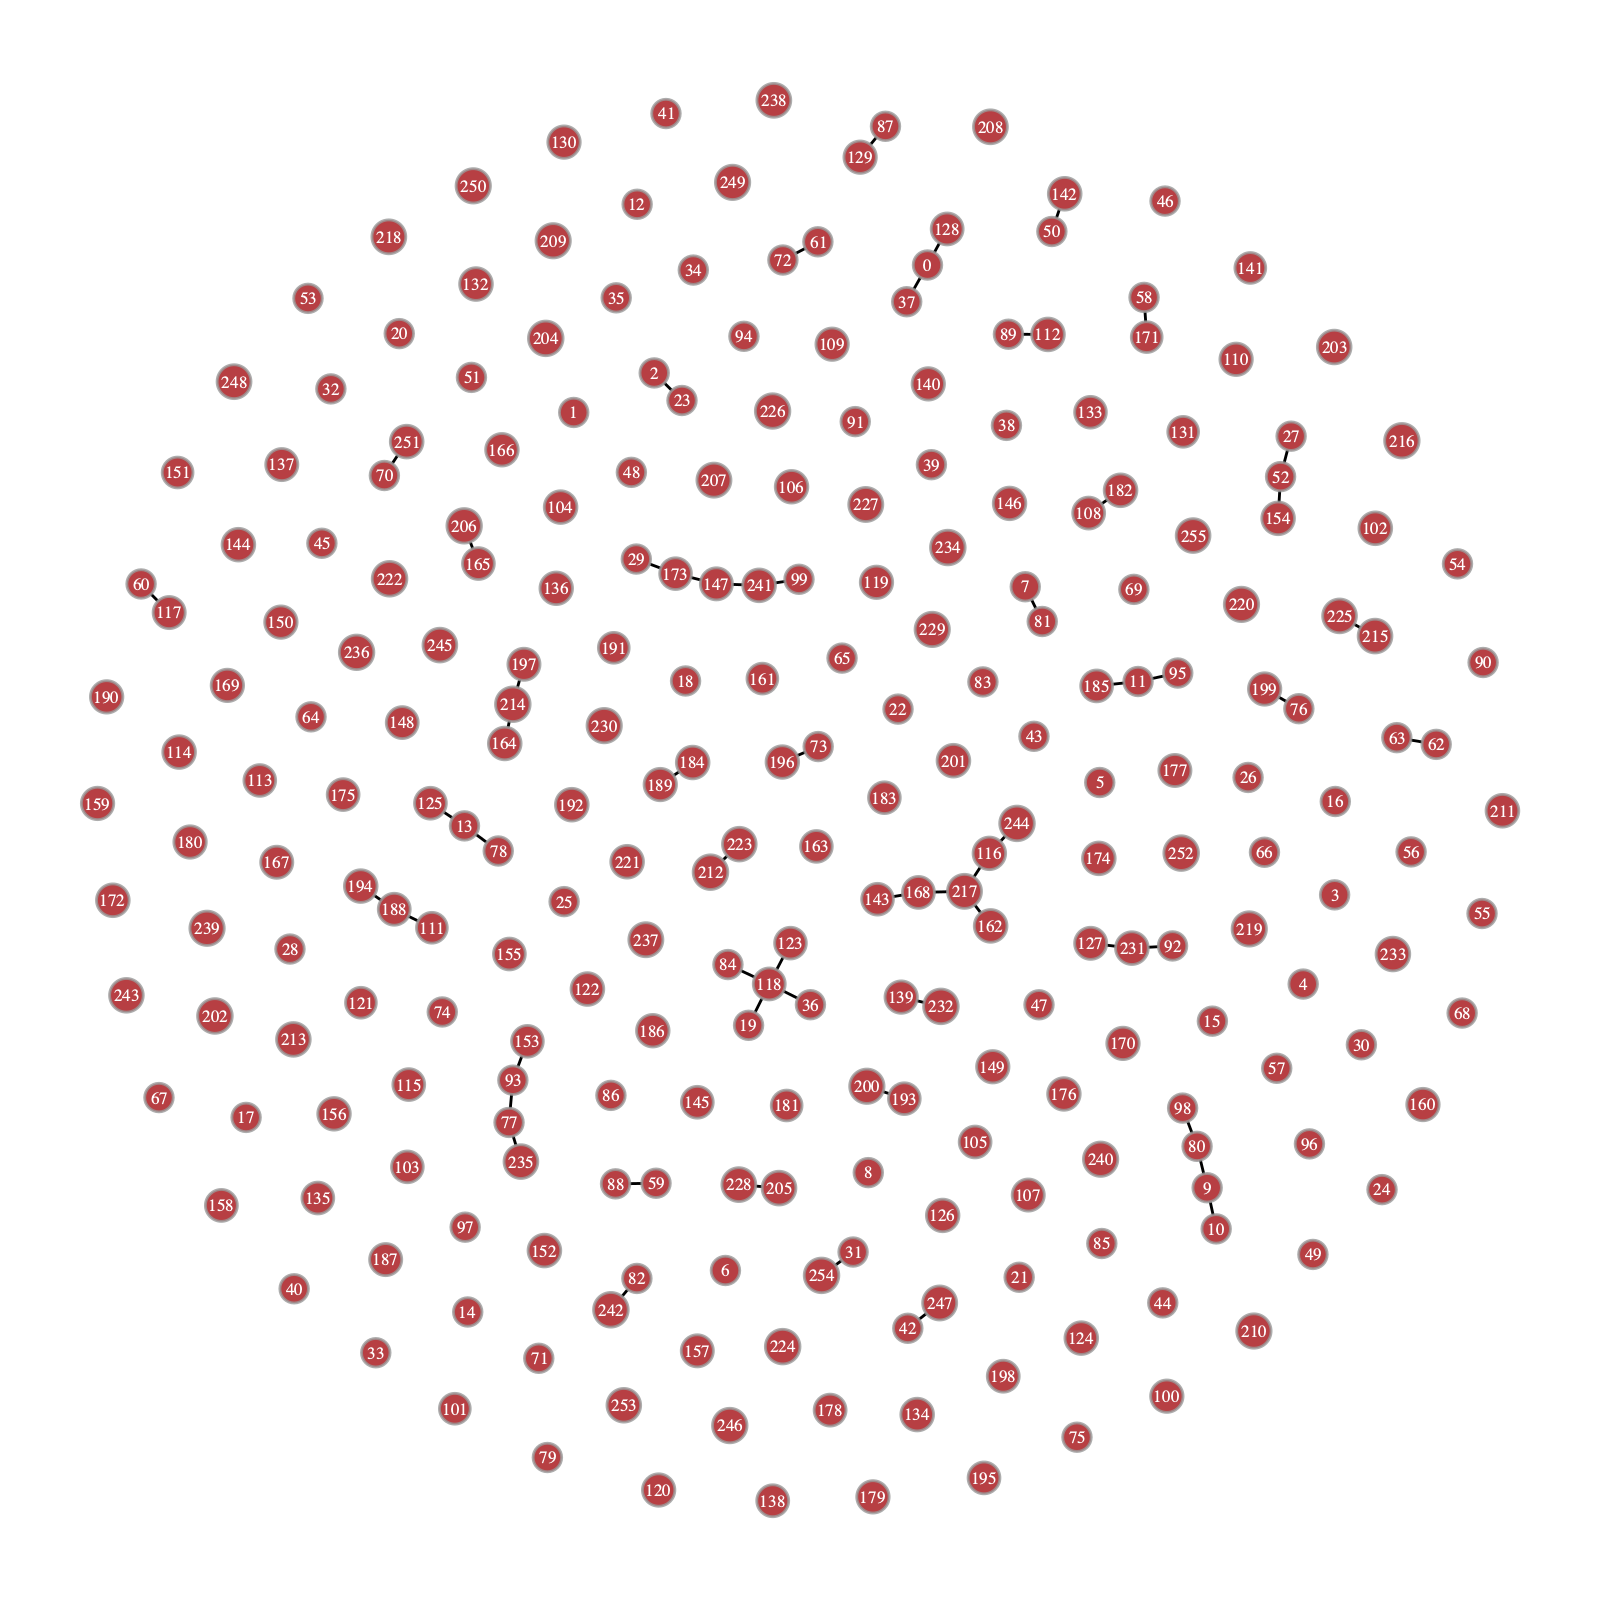
\includegraphics[width=\linewidth]{ER_Examples/ER_SP.png}
  \caption*{$p$ $\leq$ $\frac{1-\epsilon}{n}$}
\endminipage\hfill
\minipage{0.31\textwidth}
  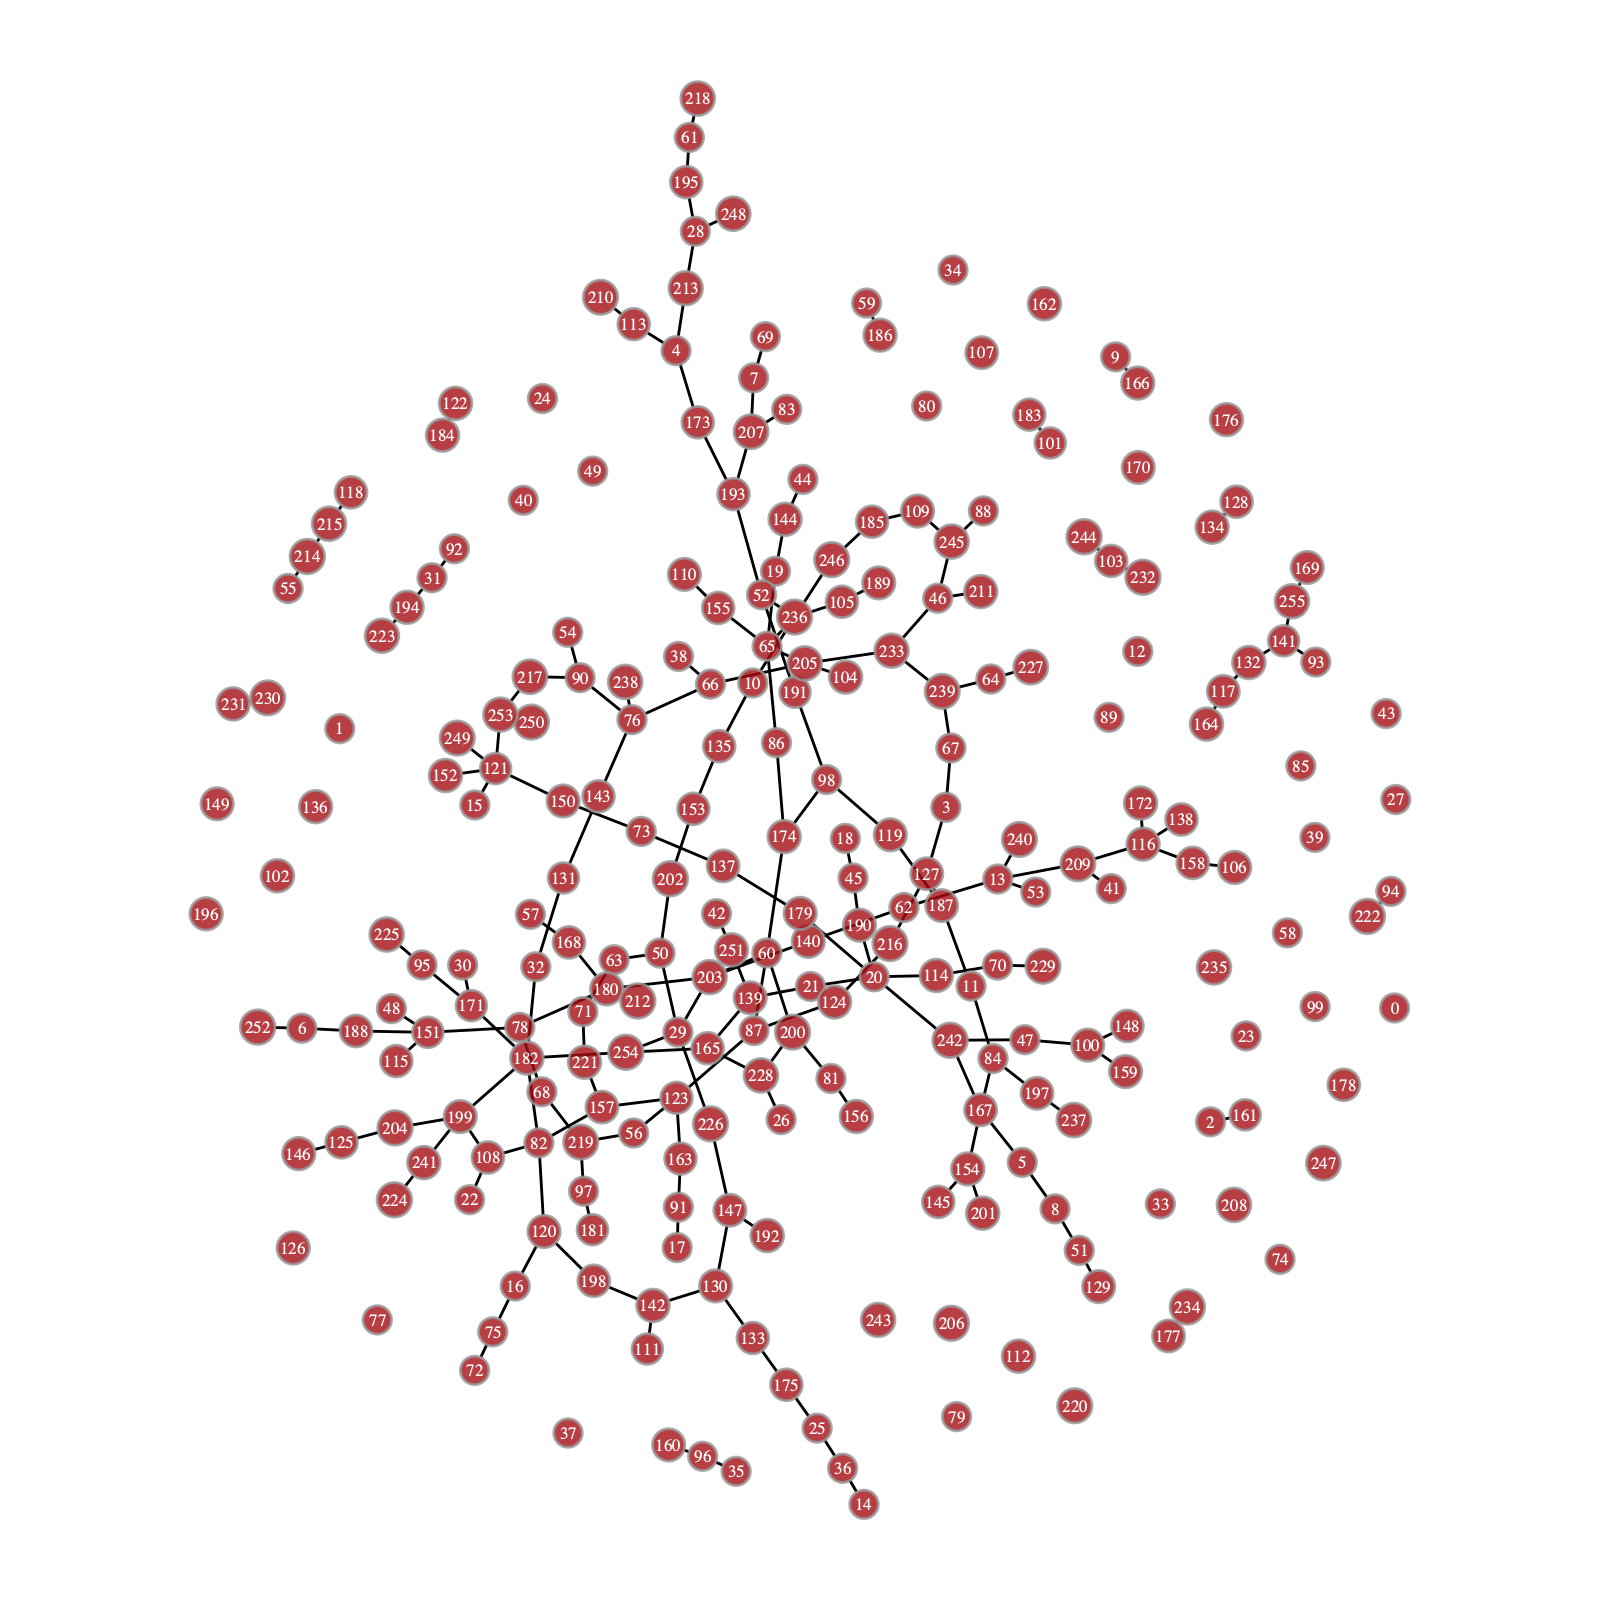
\includegraphics[width=\linewidth]{ER_Examples/ER_GC.png}
  \caption*{$p$ $\geq$ $\frac{1+\epsilon}{n}$}
\endminipage\hfill
\minipage{0.31\textwidth}%
  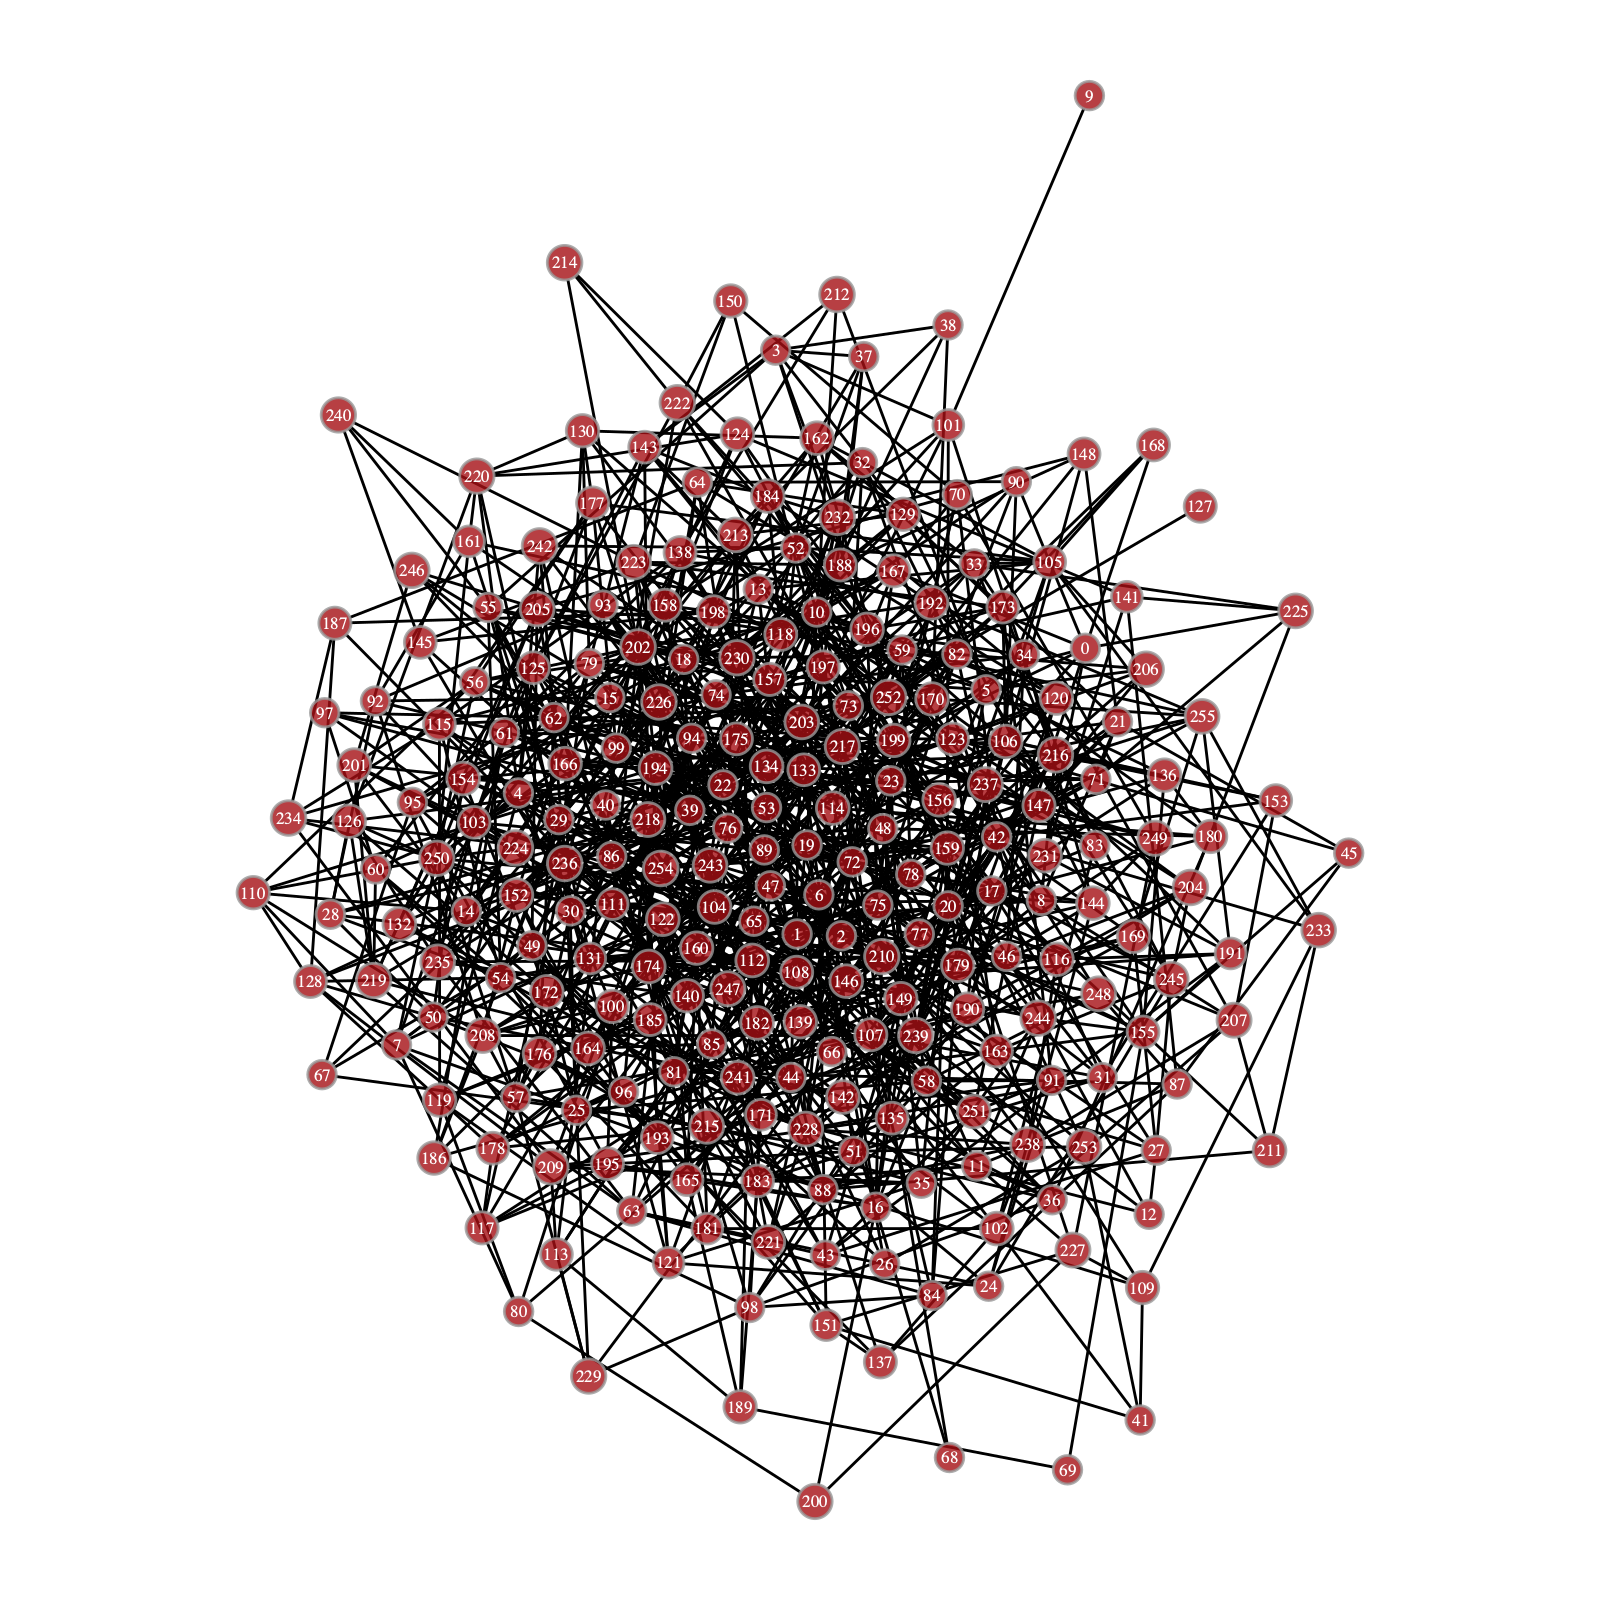
\includegraphics[width=\linewidth]{ER_Examples/ER_DN.png}
  \caption*{$p$ = $\frac{\log{}n}{n}$}
\endminipage
\end{figure}



\section{Opinion Dynamic Simulator}
Il software sviluppato fornisce degli strumenti utili a riprodurre le dinamiche descritte al fine di indagare legami inespressi che intercorrono tra alcune topologie e valori di bias.\\*
Il linguaggio principale scelto per lo sviluppo del software è Python. Le motivazioni dietro tale scelta risiedono non soltanto nella grande diffusione e nel grande supporto di cui questo linguaggio gode, ma anche dalla presenza di numerosi moduli che permettono di rappresentare ed interagire al meglio con i grafi, strutture attraverso le quali viene rappresentata la rete sociale.
Tra i vari moduli disponibili è stato scelto Graph-Tool. Tra i punti di forza di questo modulo si annoverano una precisa modellazione di tali strutture, con possibilità di aggiungere proprietà personalizzate su vertici e archi nonchè numerose funzioni di generazione e rappresentazione di alcune topologie tipiche dei grafi, quali Paths, Cicli e Cliques. Il vero punto di forza di Graph-Tool è però la sua velocità, ottenuta grazie alla possibilità di eseguire molte di queste funzioni non in Python, bensì in C, linguaggio di livello più basso e perciò più rapido nell'esecuzione di alcune istruzioni fondamentali.\\*
Alcune topologie non presenti nativamente nel modulo, sono state personalmente riscritte utilizzando comunque le strutture di base fornite. É questo il caso dell'Ipercubo, per il quale ho scritto un algoritmo di generazione basato sull'algoritmo Bit-Fix, e del Modello di Erdős–Rényi.\\*
Partendo da tale base, è stato sviluppato il processo di simulazione vero e proprio. Tale processo necessita come input, oltre al grafo, di un oggetto (d'ora in poi definito come configurator) contenente i parametri necessari alla configurazione della simulazione, come ad esempio la dinamica adottata e il bias verso l'opinione dominante.\\* 
Al termine del processo di simulazione verranno salvate diverse informazioni, quali:
\begin{itemize}
\item Un file .XML contenente la serializzazione del grafo, cosi che possa essere facilmente ricostruito e riutilizzato.
\item Un file .XML contenente le informazioni di configurazione e il risultato (numero di step) della simulazione.
\item Una rappresentazione grafica del grafo in formato .PNG
\item Una cartella contenente dei file .PNG che mostrano l'andamento evolutivo della simulazione.
\end{itemize}
Al fine di ottenere dei dati quanto più possibile affidabili e limitare l'aleatorietà di tali processi, il software dispone inoltre di un modulo volto all'esecuzione di test. In questo contesto per test si intende l'esecuzione ripetuta di una simulazione, mantenendo invariati i parametri di configurazione e la struttura del grafo. Così come le simulazioni, anche i test necessitano di una configurazione che include, oltre al numero di iterazioni da effettuare, l'oggetto configurator riferito alle simulazioni eseguite nel test.
Ponendo come obiettivo quello di velocizzare l'esecuzione di un test e ridurre la dimensione dell'output, soprattutto per grafi molto densi e popolati, l'esecuzione di un test non comporta il salvataggio di tutte le informazioni relative alle singole simulazioni, ma solamente:
\begin{itemize}
\item Un file .XML contenente la serializzazione del grafo, cosi che possa essere facilmente ricostruito e riutilizzato.
\item Un file .XML contenente le informazioni di configurazione del test, i risultati di ogni singola simulazione, la media di tali valori e la deviazione standard.
\item Una rappresentazione grafica del grafo in formato .PNG.
\end{itemize}
Considerando la durata media di un test composto da 100 simulazioni, eseguito su un grafo particolarmente impegnativo, ad esempio con $2^{12^{\mathrm{}}}$ vertici, ho scelto di inserire un modulo che permettesse di riunificare molteplici test pre-eseguiti, utilizzando come dataset l'insieme delle simulazioni eseguite e ricalcolando correttamente la media e la deviazione standard.\\*
In questo modo è possibile suddividere un test composto da 100 simulazioni in 10 test indipendenti, da 10 simulazioni ognuno, permettendo così di ridurre sensibilmente lo stress computazionale inflitto alla macchina sul quale viene eseguito.\\
La scelta del formato .XML è dettata dalla necessità di avere quante più informazioni possibili salvate in maniera strutturata e coerente, grazie anche alla possibilità, fornita nativamente da Python, di formattare automaticamente files in tale estensione.\\
Un ulteriore vantaggio dato dalla scelta del formato .XML è la possibilità di re-importare un grafo (tramite un metodo fornito dalla libreria graph-tool), partendo dal file ottenuto dalla serializzazione dello stesso. Questo risulta molto efficiente qualora si volessero eseguire ulteriori test/simulazioni a partire da un grafo precedentemente generato e difficilmente ricostruibile (nel caso di topologie ottenute tramite processi aleatori come nel Modello di Erdős–Rényi).
Le rappresentazioni grafiche invece sono state salvate in .PNG, un buon compromesso tra qualità dell'output e dimensione dei file stessi. Altre opzioni facilmente implementabili sono .SVG e .PDF.\\*
Il $core$ del software è rappresentato dall'algoritmo di simulazione che esegue il processo su un grafo fornito in input, aggiornando l'opinione di ogni nodo attraverso una $vertex$ $property$ definita appositamente.\\*
L'algoritmo di simulazione supporta attualmente $Voter$ $Model$ e $Majority$ $Dynamic$ ma il codice è stato modellato in modo da poter facilmente implementare, mediante un'interfaccia\footnote{Python non fornisce nativamente le interfacce, perciò è stata simulata utilizzando classi e metodi astratti.}, ulteriori dinamiche di aggiornamento.


\end{document}
